\documentclass[a4paper,14pt]{extarticle}
\usepackage{geometry}
\usepackage{fullpage}
\usepackage[parfill]{parskip}
\usepackage{graphicx}
\begin{document}
\begin{center}
\LARGE{MECH 4450 Term Project Report}\\\vspace{1em}
\Large{Project 2 (Static structure)}\\\vspace{1em}
\Large{Kong Xiangzhou 20026414}\\\vspace{1em}
\end{center}
\section{Introduction}
TODO
\section{Program modelling}
\subsection{Geometry}
The top view of original design is shown below:

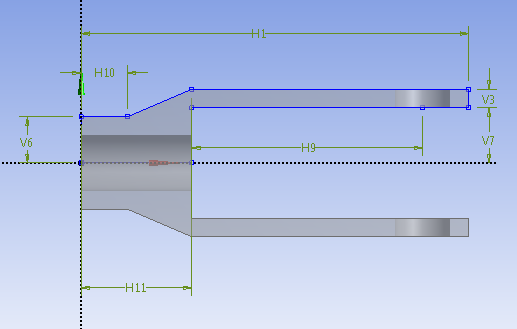
\includegraphics[width=\textwidth]{2D_ORIGIN.png}

Where diameters of all holes are $6cm$.

It is resembled as below:

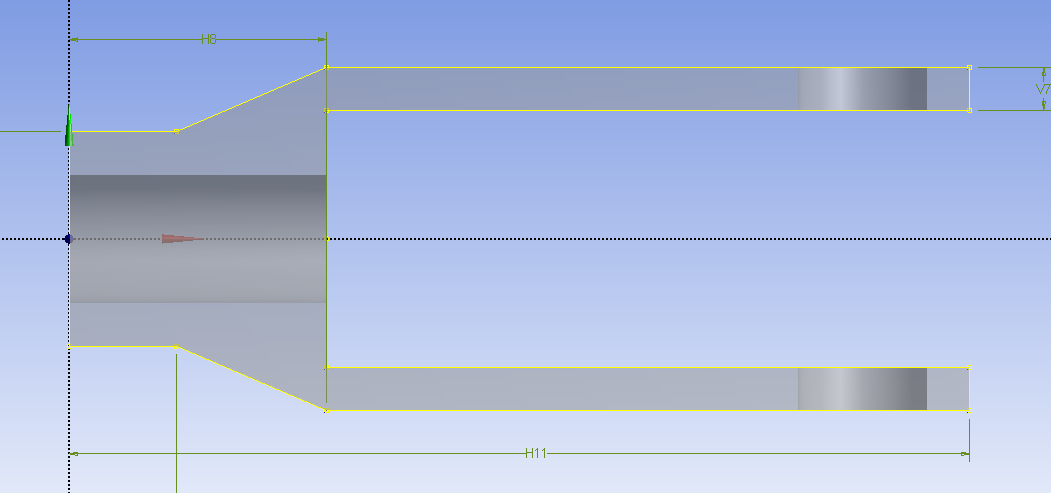
\includegraphics[width=\textwidth]{2D_S_01.PNG}

The 3D model built is then as below, where the height of the component is assumed to be $10 cm$:
\end{document}